\documentclass[1p]{elsarticle_modified}
%\bibliographystyle{elsarticle-num}

%\usepackage[colorlinks]{hyperref}
%\usepackage{abbrmath_seonhwa} %\Abb, \Ascr, \Acal ,\Abf, \Afrak
\usepackage{amsfonts}
\usepackage{amssymb}
\usepackage{amsmath}
\usepackage{amsthm}
\usepackage{scalefnt}
\usepackage{amsbsy}
\usepackage{kotex}
\usepackage{caption}
\usepackage{subfig}
\usepackage{color}
\usepackage{graphicx}
\usepackage{xcolor} %% white, black, red, green, blue, cyan, magenta, yellow
\usepackage{float}
\usepackage{setspace}
\usepackage{hyperref}

\usepackage{tikz}
\usetikzlibrary{arrows}

\usepackage{multirow}
\usepackage{array} % fixed length table
\usepackage{hhline}

%%%%%%%%%%%%%%%%%%%%%
\makeatletter
\renewcommand*\env@matrix[1][\arraystretch]{%
	\edef\arraystretch{#1}%
	\hskip -\arraycolsep
	\let\@ifnextchar\new@ifnextchar
	\array{*\c@MaxMatrixCols c}}
\makeatother %https://tex.stackexchange.com/questions/14071/how-can-i-increase-the-line-spacing-in-a-matrix
%%%%%%%%%%%%%%%

\usepackage[normalem]{ulem}

\newcommand{\msout}[1]{\ifmmode\text{\sout{\ensuremath{#1}}}\else\sout{#1}\fi}
%SOURCE: \msout is \stkout macro in https://tex.stackexchange.com/questions/20609/strikeout-in-math-mode

\newcommand{\cancel}[1]{
	\ifmmode
	{\color{red}\msout{#1}}
	\else
	{\color{red}\sout{#1}}
	\fi
}

\newcommand{\add}[1]{
	{\color{blue}\uwave{#1}}
}

\newcommand{\replace}[2]{
	\ifmmode
	{\color{red}\msout{#1}}{\color{blue}\uwave{#2}}
	\else
	{\color{red}\sout{#1}}{\color{blue}\uwave{#2}}
	\fi
}

\newcommand{\Sol}{\mathcal{S}} %segment
\newcommand{\D}{D} %diagram
\newcommand{\A}{\mathcal{A}} %arc


%%%%%%%%%%%%%%%%%%%%%%%%%%%%%5 test

\def\sl{\operatorname{\textup{SL}}(2,\Cbb)}
\def\psl{\operatorname{\textup{PSL}}(2,\Cbb)}
\def\quan{\mkern 1mu \triangleright \mkern 1mu}

\theoremstyle{definition}
\newtheorem{thm}{Theorem}[section]
\newtheorem{prop}[thm]{Proposition}
\newtheorem{lem}[thm]{Lemma}
\newtheorem{ques}[thm]{Question}
\newtheorem{cor}[thm]{Corollary}
\newtheorem{defn}[thm]{Definition}
\newtheorem{exam}[thm]{Example}
\newtheorem{rmk}[thm]{Remark}
\newtheorem{alg}[thm]{Algorithm}

\newcommand{\I}{\sqrt{-1}}
\begin{document}

%\begin{frontmatter}
%
%\title{Boundary parabolic representations of knots up to 8 crossings}
%
%%% Group authors per affiliation:
%\author{Yunhi Cho} 
%\address{Department of Mathematics, University of Seoul, Seoul, Korea}
%\ead{yhcho@uos.ac.kr}
%
%
%\author{Seonhwa Kim} %\fnref{s_kim}}
%\address{Center for Geometry and Physics, Institute for Basic Science, Pohang, 37673, Korea}
%\ead{ryeona17@ibs.re.kr}
%
%\author{Hyuk Kim}
%\address{Department of Mathematical Sciences, Seoul National University, Seoul 08826, Korea}
%\ead{hyukkim@snu.ac.kr}
%
%\author{Seokbeom Yoon}
%\address{Department of Mathematical Sciences, Seoul National University, Seoul, 08826,  Korea}
%\ead{sbyoon15@snu.ac.kr}
%
%\begin{abstract}
%We find all boundary parabolic representation of knots up to 8 crossings.
%
%\end{abstract}
%\begin{keyword}
%    \MSC[2010] 57M25 
%\end{keyword}
%
%\end{frontmatter}

%\linenumbers
%\tableofcontents
%
\newcommand\colored[1]{\textcolor{white}{\rule[-0.35ex]{0.8em}{1.4ex}}\kern-0.8em\color{red} #1}%
%\newcommand\colored[1]{\textcolor{white}{ #1}\kern-2.17ex	\textcolor{white}{ #1}\kern-1.81ex	\textcolor{white}{ #1}\kern-2.15ex\color{red}#1	}

{\Large $\underline{11a_{56}~(K11a_{56})}$}

\setlength{\tabcolsep}{10pt}
\renewcommand{\arraystretch}{1.6}
\vspace{1cm}\begin{tabular}{m{100pt}>{\centering\arraybackslash}m{274pt}}
\multirow{5}{120pt}{
	\centering
	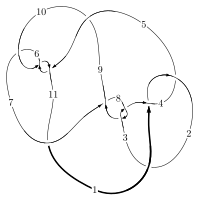
\includegraphics[width=112pt]{../../../GIT/diagram.site/Diagrams/png/305_11a_56.png}\\
\ \ \ A knot diagram\footnotemark}&
\allowdisplaybreaks
\textbf{Linearized knot diagam} \\
\cline{2-2}
 &
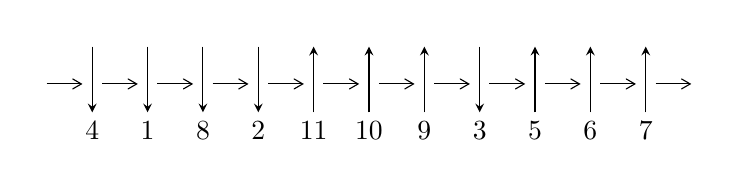
\begin{tikzpicture}[x=20pt, y=17pt]
	% nodes
	\node (C0) at (0, 0) {};
	\node (C1) at (1, 0) {};
	\node (C1U) at (1, +1) {};
	\node (C1D) at (1, -1) {4};

	\node (C2) at (2, 0) {};
	\node (C2U) at (2, +1) {};
	\node (C2D) at (2, -1) {1};

	\node (C3) at (3, 0) {};
	\node (C3U) at (3, +1) {};
	\node (C3D) at (3, -1) {8};

	\node (C4) at (4, 0) {};
	\node (C4U) at (4, +1) {};
	\node (C4D) at (4, -1) {2};

	\node (C5) at (5, 0) {};
	\node (C5U) at (5, +1) {};
	\node (C5D) at (5, -1) {11};

	\node (C6) at (6, 0) {};
	\node (C6U) at (6, +1) {};
	\node (C6D) at (6, -1) {10};

	\node (C7) at (7, 0) {};
	\node (C7U) at (7, +1) {};
	\node (C7D) at (7, -1) {9};

	\node (C8) at (8, 0) {};
	\node (C8U) at (8, +1) {};
	\node (C8D) at (8, -1) {3};

	\node (C9) at (9, 0) {};
	\node (C9U) at (9, +1) {};
	\node (C9D) at (9, -1) {5};

	\node (C10) at (10, 0) {};
	\node (C10U) at (10, +1) {};
	\node (C10D) at (10, -1) {6};

	\node (C11) at (11, 0) {};
	\node (C11U) at (11, +1) {};
	\node (C11D) at (11, -1) {7};
	\node (C12) at (12, 0) {};

	% arrows
	\draw[->,>={angle 60}]
	(C0) edge (C1) (C1) edge (C2) (C2) edge (C3) (C3) edge (C4) (C4) edge (C5) (C5) edge (C6) (C6) edge (C7) (C7) edge (C8) (C8) edge (C9) (C9) edge (C10) (C10) edge (C11) (C11) edge (C12) ;	\draw[->,>=stealth]
	(C1U) edge (C1D) (C2U) edge (C2D) (C3U) edge (C3D) (C4U) edge (C4D) (C5D) edge (C5U) (C6D) edge (C6U) (C7D) edge (C7U) (C8U) edge (C8D) (C9D) edge (C9U) (C10D) edge (C10U) (C11D) edge (C11U) ;
	\end{tikzpicture} \\
\hhline{~~} \\& 
\textbf{Solving Sequence} \\ \cline{2-2} 
 &
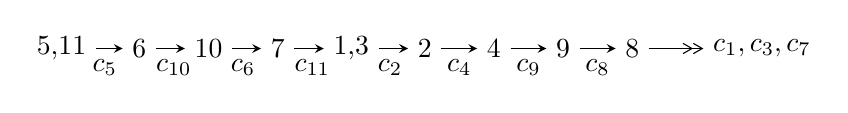
\begin{tikzpicture}[x=25pt, y=7pt]
	% node
	\node (A0) at (-1/8, 0) {5,11};
	\node (A1) at (1, 0) {6};
	\node (A2) at (2, 0) {10};
	\node (A3) at (3, 0) {7};
	\node (A4) at (65/16, 0) {1,3};
	\node (A5) at (41/8, 0) {2};
	\node (A6) at (49/8, 0) {4};
	\node (A7) at (57/8, 0) {9};
	\node (A8) at (65/8, 0) {8};
	\node (C1) at (1/2, -1) {$c_{5}$};
	\node (C2) at (3/2, -1) {$c_{10}$};
	\node (C3) at (5/2, -1) {$c_{6}$};
	\node (C4) at (7/2, -1) {$c_{11}$};
	\node (C5) at (37/8, -1) {$c_{2}$};
	\node (C6) at (45/8, -1) {$c_{4}$};
	\node (C7) at (53/8, -1) {$c_{9}$};
	\node (C8) at (61/8, -1) {$c_{8}$};
	\node (A9) at (10, 0) {$c_{1},c_{3},c_{7}$};

	% edge
	\draw[->,>=stealth]	
	(A0) edge (A1) (A1) edge (A2) (A2) edge (A3) (A3) edge (A4) (A4) edge (A5) (A5) edge (A6) (A6) edge (A7) (A7) edge (A8) ;
	\draw[->>,>={angle 60}]	
	(A8) edge (A9);
\end{tikzpicture} \\ 

\end{tabular} \\

\footnotetext{
The image of knot diagram is generated by the software ``\textbf{Draw programme}" developed by Andrew Bartholomew(\url{http://www.layer8.co.uk/maths/draw/index.htm\#Running-draw}), where we modified some parts for our purpose(\url{https://github.com/CATsTAILs/LinksPainter}).
}\phantom \\ \newline 
\centering \textbf{Ideals for irreducible components\footnotemark of $X_{\text{par}}$} 
 
\begin{align*}
I^u_{1}&=\langle 
u^{54}- u^{53}+\cdots+b+1,\;- u^{56}+2 u^{55}+\cdots+a-4,\;u^{57}-2 u^{56}+\cdots+3 u-1\rangle \\
I^u_{2}&=\langle 
b+1,\;- u^2+a- u-2,\;u^3+u^2+2 u+1\rangle \\
\\
\end{align*}
\raggedright * 2 irreducible components of $\dim_{\mathbb{C}}=0$, with total 60 representations.\\
\footnotetext{All coefficients of polynomials are rational numbers. But the coefficients are sometimes approximated in decimal forms when there is not enough margin.}
\newpage
\renewcommand{\arraystretch}{1}
\centering \section*{I. $I^u_{1}= \langle u^{54}- u^{53}+\cdots+b+1,\;- u^{56}+2 u^{55}+\cdots+a-4,\;u^{57}-2 u^{56}+\cdots+3 u-1 \rangle$}
\flushleft \textbf{(i) Arc colorings}\\
\begin{tabular}{m{7pt} m{180pt} m{7pt} m{180pt} }
\flushright $a_{5}=$&$\begin{pmatrix}1\\0\end{pmatrix}$ \\
\flushright $a_{11}=$&$\begin{pmatrix}0\\u\end{pmatrix}$ \\
\flushright $a_{6}=$&$\begin{pmatrix}1\\- u^2\end{pmatrix}$ \\
\flushright $a_{10}=$&$\begin{pmatrix}- u\\u^3+u\end{pmatrix}$ \\
\flushright $a_{7}=$&$\begin{pmatrix}u^2+1\\- u^4-2 u^2\end{pmatrix}$ \\
\flushright $a_{1}=$&$\begin{pmatrix}u^5+2 u^3+u\\- u^7-3 u^5-2 u^3+u\end{pmatrix}$ \\
\flushright $a_{3}=$&$\begin{pmatrix}u^{56}-2 u^{55}+\cdots+2 u+4\\- u^{54}+u^{53}+\cdots- u-1\end{pmatrix}$ \\
\flushright $a_{2}=$&$\begin{pmatrix}u^{56}-2 u^{55}+\cdots+3 u+3\\- u^{54}+u^{53}+\cdots- u-1\end{pmatrix}$ \\
\flushright $a_{4}=$&$\begin{pmatrix}u^{56}-2 u^{55}+\cdots+4 u+3\\- u^{54}+u^{53}+\cdots+2 u^2-1\end{pmatrix}$ \\
\flushright $a_{9}=$&$\begin{pmatrix}- u^3-2 u\\u^3+u\end{pmatrix}$ \\
\flushright $a_{8}=$&$\begin{pmatrix}- u^{10}-5 u^8-8 u^6-3 u^4+3 u^2+1\\u^{10}+4 u^8+5 u^6-3 u^2\end{pmatrix}$\\ \flushright $a_{8}=$&$\begin{pmatrix}- u^{10}-5 u^8-8 u^6-3 u^4+3 u^2+1\\u^{10}+4 u^8+5 u^6-3 u^2\end{pmatrix}$\\&\end{tabular}
\flushleft \textbf{(ii) Obstruction class $= -1$}\\~\\
\flushleft \textbf{(iii) Cusp Shapes $= - u^{56}+2 u^{55}+\cdots-8 u-9$}\\~\\
\newpage\renewcommand{\arraystretch}{1}
\flushleft \textbf{(iv) u-Polynomials at the component}\newline \\
\begin{tabular}{m{50pt}|m{274pt}}
Crossings & \hspace{64pt}u-Polynomials at each crossing \\
\hline $$\begin{aligned}c_{1},c_{4}\end{aligned}$$&$\begin{aligned}
&u^{57}-4 u^{56}+\cdots-4 u+1
\end{aligned}$\\
\hline $$\begin{aligned}c_{2}\end{aligned}$$&$\begin{aligned}
&u^{57}+30 u^{56}+\cdots+4 u+1
\end{aligned}$\\
\hline $$\begin{aligned}c_{3},c_{8}\end{aligned}$$&$\begin{aligned}
&u^{57}- u^{56}+\cdots+4 u+8
\end{aligned}$\\
\hline $$\begin{aligned}c_{5},c_{6},c_{10}\end{aligned}$$&$\begin{aligned}
&u^{57}+2 u^{56}+\cdots+3 u+1
\end{aligned}$\\
\hline $$\begin{aligned}c_{7}\end{aligned}$$&$\begin{aligned}
&u^{57}-21 u^{56}+\cdots-496 u+64
\end{aligned}$\\
\hline $$\begin{aligned}c_{9},c_{11}\end{aligned}$$&$\begin{aligned}
&u^{57}-2 u^{56}+\cdots-3 u+9
\end{aligned}$\\
\hline
\end{tabular}\\~\\
\newpage\renewcommand{\arraystretch}{1}
\flushleft \textbf{(v) Riley Polynomials at the component}\newline \\
\begin{tabular}{m{50pt}|m{274pt}}
Crossings & \hspace{64pt}Riley Polynomials at each crossing \\
\hline $$\begin{aligned}c_{1},c_{4}\end{aligned}$$&$\begin{aligned}
&y^{57}-30 y^{56}+\cdots+4 y-1
\end{aligned}$\\
\hline $$\begin{aligned}c_{2}\end{aligned}$$&$\begin{aligned}
&y^{57}-2 y^{56}+\cdots-24 y-1
\end{aligned}$\\
\hline $$\begin{aligned}c_{3},c_{8}\end{aligned}$$&$\begin{aligned}
&y^{57}+21 y^{56}+\cdots-496 y-64
\end{aligned}$\\
\hline $$\begin{aligned}c_{5},c_{6},c_{10}\end{aligned}$$&$\begin{aligned}
&y^{57}+48 y^{56}+\cdots+23 y-1
\end{aligned}$\\
\hline $$\begin{aligned}c_{7}\end{aligned}$$&$\begin{aligned}
&y^{57}+25 y^{56}+\cdots+134400 y-4096
\end{aligned}$\\
\hline $$\begin{aligned}c_{9},c_{11}\end{aligned}$$&$\begin{aligned}
&y^{57}-32 y^{56}+\cdots+1719 y-81
\end{aligned}$\\
\hline
\end{tabular}\\~\\
\newpage\flushleft \textbf{(vi) Complex Volumes and Cusp Shapes}
$$\begin{array}{c|c|c}  
\text{Solutions to }I^u_{1}& \I (\text{vol} + \sqrt{-1}CS) & \text{Cusp shape}\\
 \hline 
\begin{aligned}
u &= \phantom{-}0.339361 + 1.049480 I \\
a &= \phantom{-}0.50854 - 1.48654 I \\
b &= -1.48903 + 0.96739 I\end{aligned}
 & -1.26618 - 6.23330 I & \phantom{-0.000000 } 0 \\ \hline\begin{aligned}
u &= \phantom{-}0.339361 - 1.049480 I \\
a &= \phantom{-}0.50854 + 1.48654 I \\
b &= -1.48903 - 0.96739 I\end{aligned}
 & -1.26618 + 6.23330 I & \phantom{-0.000000 } 0 \\ \hline\begin{aligned}
u &= -0.245002 + 1.131380 I \\
a &= -0.32304 - 1.42186 I \\
b &= \phantom{-}0.208942 + 0.592370 I\end{aligned}
 & -3.18295 + 0.59460 I & \phantom{-0.000000 } 0 \\ \hline\begin{aligned}
u &= -0.245002 - 1.131380 I \\
a &= -0.32304 + 1.42186 I \\
b &= \phantom{-}0.208942 - 0.592370 I\end{aligned}
 & -3.18295 - 0.59460 I & \phantom{-0.000000 } 0 \\ \hline\begin{aligned}
u &= \phantom{-}0.317804 + 1.113660 I \\
a &= -0.301756 + 1.180030 I \\
b &= \phantom{-}1.38215 - 0.87035 I\end{aligned}
 & \phantom{-}1.12994 - 1.12326 I & \phantom{-0.000000 } 0 \\ \hline\begin{aligned}
u &= \phantom{-}0.317804 - 1.113660 I \\
a &= -0.301756 - 1.180030 I \\
b &= \phantom{-}1.38215 + 0.87035 I\end{aligned}
 & \phantom{-}1.12994 + 1.12326 I & \phantom{-0.000000 } 0 \\ \hline\begin{aligned}
u &= \phantom{-}0.799224 + 0.161136 I \\
a &= \phantom{-}3.09156 + 0.85984 I \\
b &= -1.72076 - 1.24432 I\end{aligned}
 & \phantom{-}1.44780 + 10.42440 I & \phantom{-}2.90383 - 7.96893 I \\ \hline\begin{aligned}
u &= \phantom{-}0.799224 - 0.161136 I \\
a &= \phantom{-}3.09156 - 0.85984 I \\
b &= -1.72076 + 1.24432 I\end{aligned}
 & \phantom{-}1.44780 - 10.42440 I & \phantom{-}2.90383 + 7.96893 I \\ \hline\begin{aligned}
u &= \phantom{-}0.806026 + 0.024229 I \\
a &= -0.524270 - 0.510392 I \\
b &= \phantom{-}0.297226 + 0.891673 I\end{aligned}
 & \phantom{-}7.00743 + 2.64990 I & \phantom{-}8.23772 - 3.33458 I \\ \hline\begin{aligned}
u &= \phantom{-}0.806026 - 0.024229 I \\
a &= -0.524270 + 0.510392 I \\
b &= \phantom{-}0.297226 - 0.891673 I\end{aligned}
 & \phantom{-}7.00743 - 2.64990 I & \phantom{-}8.23772 + 3.33458 I\\
 \hline 
 \end{array}$$\newpage$$\begin{array}{c|c|c}  
\text{Solutions to }I^u_{1}& \I (\text{vol} + \sqrt{-1}CS) & \text{Cusp shape}\\
 \hline 
\begin{aligned}
u &= \phantom{-}0.787966 + 0.130536 I \\
a &= -2.57577 - 0.95104 I \\
b &= \phantom{-}1.42239 + 1.23954 I\end{aligned}
 & \phantom{-}4.10218 + 5.18574 I & \phantom{-}6.42318 - 4.39381 I \\ \hline\begin{aligned}
u &= \phantom{-}0.787966 - 0.130536 I \\
a &= -2.57577 + 0.95104 I \\
b &= \phantom{-}1.42239 - 1.23954 I\end{aligned}
 & \phantom{-}4.10218 - 5.18574 I & \phantom{-}6.42318 + 4.39381 I \\ \hline\begin{aligned}
u &= \phantom{-}0.226143 + 1.198470 I \\
a &= -0.29741 - 1.54674 I \\
b &= -1.71216 + 1.04442 I\end{aligned}
 & -3.91254 + 1.67555 I & \phantom{-0.000000 } 0 \\ \hline\begin{aligned}
u &= \phantom{-}0.226143 - 1.198470 I \\
a &= -0.29741 + 1.54674 I \\
b &= -1.71216 - 1.04442 I\end{aligned}
 & -3.91254 - 1.67555 I & \phantom{-0.000000 } 0 \\ \hline\begin{aligned}
u &= -0.754570 + 0.135098 I \\
a &= -1.92141 + 1.62306 I \\
b &= \phantom{-}0.580662 - 0.892200 I\end{aligned}
 & -0.25463 - 4.33211 I & \phantom{-}1.62345 + 4.63416 I \\ \hline\begin{aligned}
u &= -0.754570 - 0.135098 I \\
a &= -1.92141 - 1.62306 I \\
b &= \phantom{-}0.580662 + 0.892200 I\end{aligned}
 & -0.25463 + 4.33211 I & \phantom{-}1.62345 - 4.63416 I \\ \hline\begin{aligned}
u &= -0.338013 + 0.681571 I \\
a &= \phantom{-}0.642106 - 0.604854 I \\
b &= -0.849512 + 0.966860 I\end{aligned}
 & -2.04198 - 6.13465 I & -0.96110 + 7.52026 I \\ \hline\begin{aligned}
u &= -0.338013 - 0.681571 I \\
a &= \phantom{-}0.642106 + 0.604854 I \\
b &= -0.849512 - 0.966860 I\end{aligned}
 & -2.04198 + 6.13465 I & -0.96110 - 7.52026 I \\ \hline\begin{aligned}
u &= \phantom{-}0.722838 + 0.126778 I \\
a &= \phantom{-}2.54617 + 1.95088 I \\
b &= -1.31528 - 1.75485 I\end{aligned}
 & -0.80005 + 1.75324 I & \phantom{-}2.03009 - 4.15615 I \\ \hline\begin{aligned}
u &= \phantom{-}0.722838 - 0.126778 I \\
a &= \phantom{-}2.54617 - 1.95088 I \\
b &= -1.31528 + 1.75485 I\end{aligned}
 & -0.80005 - 1.75324 I & \phantom{-}2.03009 + 4.15615 I\\
 \hline 
 \end{array}$$\newpage$$\begin{array}{c|c|c}  
\text{Solutions to }I^u_{1}& \I (\text{vol} + \sqrt{-1}CS) & \text{Cusp shape}\\
 \hline 
\begin{aligned}
u &= -0.275696 + 1.237520 I \\
a &= \phantom{-}0.808387 + 0.975749 I \\
b &= -0.556151 - 0.097923 I\end{aligned}
 & -1.78635 - 3.24178 I & \phantom{-0.000000 } 0 \\ \hline\begin{aligned}
u &= -0.275696 - 1.237520 I \\
a &= \phantom{-}0.808387 - 0.975749 I \\
b &= -0.556151 + 0.097923 I\end{aligned}
 & -1.78635 + 3.24178 I & \phantom{-0.000000 } 0 \\ \hline\begin{aligned}
u &= \phantom{-}0.353003 + 1.235470 I \\
a &= \phantom{-}0.259194 + 0.074469 I \\
b &= \phantom{-}0.608563 - 0.823394 I\end{aligned}
 & \phantom{-}3.27082 + 1.52614 I & \phantom{-0.000000 } 0 \\ \hline\begin{aligned}
u &= \phantom{-}0.353003 - 1.235470 I \\
a &= \phantom{-}0.259194 - 0.074469 I \\
b &= \phantom{-}0.608563 + 0.823394 I\end{aligned}
 & \phantom{-}3.27082 - 1.52614 I & \phantom{-0.000000 } 0 \\ \hline\begin{aligned}
u &= -0.664926 + 0.248231 I \\
a &= -0.53582 + 1.91639 I \\
b &= -0.321007 - 0.845457 I\end{aligned}
 & -0.56153 + 2.51315 I & \phantom{-}1.83697 - 2.48665 I \\ \hline\begin{aligned}
u &= -0.664926 - 0.248231 I \\
a &= -0.53582 - 1.91639 I \\
b &= -0.321007 + 0.845457 I\end{aligned}
 & -0.56153 - 2.51315 I & \phantom{-}1.83697 + 2.48665 I \\ \hline\begin{aligned}
u &= -0.704230 + 0.061019 I \\
a &= \phantom{-}1.64700 - 0.65736 I \\
b &= -0.525612 + 0.326561 I\end{aligned}
 & \phantom{-}1.82968 - 0.29846 I & \phantom{-}5.16983 - 0.57329 I \\ \hline\begin{aligned}
u &= -0.704230 - 0.061019 I \\
a &= \phantom{-}1.64700 + 0.65736 I \\
b &= -0.525612 - 0.326561 I\end{aligned}
 & \phantom{-}1.82968 + 0.29846 I & \phantom{-}5.16983 + 0.57329 I \\ \hline\begin{aligned}
u &= \phantom{-}0.355735 + 1.276270 I \\
a &= -0.681670 + 0.406147 I \\
b &= -0.007104 + 0.903876 I\end{aligned}
 & \phantom{-}2.96572 + 6.83199 I & \phantom{-0.000000 } 0 \\ \hline\begin{aligned}
u &= \phantom{-}0.355735 - 1.276270 I \\
a &= -0.681670 - 0.406147 I \\
b &= -0.007104 - 0.903876 I\end{aligned}
 & \phantom{-}2.96572 - 6.83199 I & \phantom{-0.000000 } 0\\
 \hline 
 \end{array}$$\newpage$$\begin{array}{c|c|c}  
\text{Solutions to }I^u_{1}& \I (\text{vol} + \sqrt{-1}CS) & \text{Cusp shape}\\
 \hline 
\begin{aligned}
u &= -0.294328 + 1.319490 I \\
a &= \phantom{-}1.338980 + 0.220264 I \\
b &= -0.580535 + 0.617472 I\end{aligned}
 & -2.52174 - 3.91370 I & \phantom{-0.000000 } 0 \\ \hline\begin{aligned}
u &= -0.294328 - 1.319490 I \\
a &= \phantom{-}1.338980 - 0.220264 I \\
b &= -0.580535 - 0.617472 I\end{aligned}
 & -2.52174 + 3.91370 I & \phantom{-0.000000 } 0 \\ \hline\begin{aligned}
u &= -0.181659 + 1.350590 I \\
a &= \phantom{-}0.400207 - 0.673731 I \\
b &= \phantom{-}0.475022 + 0.135856 I\end{aligned}
 & -3.91953 - 3.45367 I & \phantom{-0.000000 } 0 \\ \hline\begin{aligned}
u &= -0.181659 - 1.350590 I \\
a &= \phantom{-}0.400207 + 0.673731 I \\
b &= \phantom{-}0.475022 - 0.135856 I\end{aligned}
 & -3.91953 + 3.45367 I & \phantom{-0.000000 } 0 \\ \hline\begin{aligned}
u &= \phantom{-}0.308057 + 1.342450 I \\
a &= \phantom{-}2.07004 - 0.68307 I \\
b &= -1.21623 - 2.16373 I\end{aligned}
 & -5.43045 + 5.50488 I & \phantom{-0.000000 } 0 \\ \hline\begin{aligned}
u &= \phantom{-}0.308057 - 1.342450 I \\
a &= \phantom{-}2.07004 + 0.68307 I \\
b &= -1.21623 + 2.16373 I\end{aligned}
 & -5.43045 - 5.50488 I & \phantom{-0.000000 } 0 \\ \hline\begin{aligned}
u &= -0.040540 + 1.380290 I \\
a &= \phantom{-}0.437295 - 0.786403 I \\
b &= \phantom{-}0.388863 - 1.268110 I\end{aligned}
 & -5.57754 - 2.56020 I & \phantom{-0.000000 } 0 \\ \hline\begin{aligned}
u &= -0.040540 - 1.380290 I \\
a &= \phantom{-}0.437295 + 0.786403 I \\
b &= \phantom{-}0.388863 + 1.268110 I\end{aligned}
 & -5.57754 + 2.56020 I & \phantom{-0.000000 } 0 \\ \hline\begin{aligned}
u &= -0.321142 + 1.347280 I \\
a &= -1.81984 - 0.00606 I \\
b &= \phantom{-}0.797242 - 1.062560 I\end{aligned}
 & -4.92507 - 8.23091 I & \phantom{-0.000000 } 0 \\ \hline\begin{aligned}
u &= -0.321142 - 1.347280 I \\
a &= -1.81984 + 0.00606 I \\
b &= \phantom{-}0.797242 + 1.062560 I\end{aligned}
 & -4.92507 + 8.23091 I & \phantom{-0.000000 } 0\\
 \hline 
 \end{array}$$\newpage$$\begin{array}{c|c|c}  
\text{Solutions to }I^u_{1}& \I (\text{vol} + \sqrt{-1}CS) & \text{Cusp shape}\\
 \hline 
\begin{aligned}
u &= \phantom{-}0.010128 + 1.388520 I \\
a &= -0.665649 + 0.739671 I \\
b &= \phantom{-}0.02872 + 1.83602 I\end{aligned}
 & -9.28405 + 1.35733 I & \phantom{-0.000000 } 0 \\ \hline\begin{aligned}
u &= \phantom{-}0.010128 - 1.388520 I \\
a &= -0.665649 - 0.739671 I \\
b &= \phantom{-}0.02872 - 1.83602 I\end{aligned}
 & -9.28405 - 1.35733 I & \phantom{-0.000000 } 0 \\ \hline\begin{aligned}
u &= \phantom{-}0.337618 + 1.347450 I \\
a &= -1.76632 + 1.05829 I \\
b &= \phantom{-}1.40418 + 1.48266 I\end{aligned}
 & -0.55115 + 9.25140 I & \phantom{-0.000000 } 0 \\ \hline\begin{aligned}
u &= \phantom{-}0.337618 - 1.347450 I \\
a &= -1.76632 - 1.05829 I \\
b &= \phantom{-}1.40418 - 1.48266 I\end{aligned}
 & -0.55115 - 9.25140 I & \phantom{-0.000000 } 0 \\ \hline\begin{aligned}
u &= \phantom{-}0.086152 + 0.593036 I \\
a &= -0.86026 - 1.12969 I \\
b &= -0.349711 + 1.132030 I\end{aligned}
 & -3.25990 + 1.13842 I & -4.67839 - 1.12304 I \\ \hline\begin{aligned}
u &= \phantom{-}0.086152 - 0.593036 I \\
a &= -0.86026 + 1.12969 I \\
b &= -0.349711 - 1.132030 I\end{aligned}
 & -3.25990 - 1.13842 I & -4.67839 + 1.12304 I \\ \hline\begin{aligned}
u &= -0.268783 + 1.376140 I \\
a &= -1.251340 + 0.579944 I \\
b &= -0.053457 - 1.081820 I\end{aligned}
 & -5.67983 - 0.88312 I & \phantom{-0.000000 } 0 \\ \hline\begin{aligned}
u &= -0.268783 - 1.376140 I \\
a &= -1.251340 - 0.579944 I \\
b &= -0.053457 + 1.081820 I\end{aligned}
 & -5.67983 + 0.88312 I & \phantom{-0.000000 } 0 \\ \hline\begin{aligned}
u &= \phantom{-}0.340495 + 1.364500 I \\
a &= \phantom{-}1.93564 - 1.27843 I \\
b &= -1.80297 - 1.45511 I\end{aligned}
 & -3.3664 + 14.5406 I & \phantom{-0.000000 } 0 \\ \hline\begin{aligned}
u &= \phantom{-}0.340495 - 1.364500 I \\
a &= \phantom{-}1.93564 + 1.27843 I \\
b &= -1.80297 + 1.45511 I\end{aligned}
 & -3.3664 - 14.5406 I & \phantom{-0.000000 } 0\\
 \hline 
 \end{array}$$\newpage$$\begin{array}{c|c|c}  
\text{Solutions to }I^u_{1}& \I (\text{vol} + \sqrt{-1}CS) & \text{Cusp shape}\\
 \hline 
\begin{aligned}
u &= -0.279491 + 0.522898 I \\
a &= -0.1114230 + 0.0411162 I \\
b &= \phantom{-}0.664100 - 0.647028 I\end{aligned}
 & \phantom{-}0.29336 - 1.71892 I & \phantom{-}2.35747 + 4.28522 I \\ \hline\begin{aligned}
u &= -0.279491 - 0.522898 I \\
a &= -0.1114230 - 0.0411162 I \\
b &= \phantom{-}0.664100 + 0.647028 I\end{aligned}
 & \phantom{-}0.29336 + 1.71892 I & \phantom{-}2.35747 - 4.28522 I \\ \hline\begin{aligned}
u &= -0.04491 + 1.42071 I \\
a &= -0.362172 + 0.648626 I \\
b &= -0.88717 + 1.55692 I\end{aligned}
 & -8.60971 - 7.06322 I & \phantom{-0.000000 } 0 \\ \hline\begin{aligned}
u &= -0.04491 - 1.42071 I \\
a &= -0.362172 - 0.648626 I \\
b &= -0.88717 - 1.55692 I\end{aligned}
 & -8.60971 + 7.06322 I & \phantom{-0.000000 } 0 \\ \hline\begin{aligned}
u &= -0.475182 + 0.281427 I \\
a &= \phantom{-}0.033922 - 1.111620 I \\
b &= \phantom{-}0.503597 + 0.110254 I\end{aligned}
 & \phantom{-}1.12264 - 1.10520 I & \phantom{-}5.95384 + 5.07623 I \\ \hline\begin{aligned}
u &= -0.475182 - 0.281427 I \\
a &= \phantom{-}0.033922 + 1.111620 I \\
b &= \phantom{-}0.503597 - 0.110254 I\end{aligned}
 & \phantom{-}1.12264 + 1.10520 I & \phantom{-}5.95384 - 5.07623 I \\ \hline\begin{aligned}
u &= \phantom{-}0.195845\phantom{ +0.000000I} \\
a &= \phantom{-}3.55820\phantom{ +0.000000I} \\
b &= -0.749956\phantom{ +0.000000I}\end{aligned}
 & -1.30246\phantom{ +0.000000I} & -9.05740\phantom{ +0.000000I}\\
 \hline 
 \end{array}$$\newpage\newpage\renewcommand{\arraystretch}{1}
\centering \section*{II. $I^u_{2}= \langle b+1,\;- u^2+a- u-2,\;u^3+u^2+2 u+1 \rangle$}
\flushleft \textbf{(i) Arc colorings}\\
\begin{tabular}{m{7pt} m{180pt} m{7pt} m{180pt} }
\flushright $a_{5}=$&$\begin{pmatrix}1\\0\end{pmatrix}$ \\
\flushright $a_{11}=$&$\begin{pmatrix}0\\u\end{pmatrix}$ \\
\flushright $a_{6}=$&$\begin{pmatrix}1\\- u^2\end{pmatrix}$ \\
\flushright $a_{10}=$&$\begin{pmatrix}- u\\- u^2- u-1\end{pmatrix}$ \\
\flushright $a_{7}=$&$\begin{pmatrix}u^2+1\\- u^2- u-1\end{pmatrix}$ \\
\flushright $a_{1}=$&$\begin{pmatrix}-1\\0\end{pmatrix}$ \\
\flushright $a_{3}=$&$\begin{pmatrix}u^2+u+2\\-1\end{pmatrix}$ \\
\flushright $a_{2}=$&$\begin{pmatrix}u^2+u+1\\-1\end{pmatrix}$ \\
\flushright $a_{4}=$&$\begin{pmatrix}u^2+u+2\\-1\end{pmatrix}$ \\
\flushright $a_{9}=$&$\begin{pmatrix}u^2+1\\- u^2- u-1\end{pmatrix}$ \\
\flushright $a_{8}=$&$\begin{pmatrix}u^2+1\\- u^2- u-1\end{pmatrix}$\\ \flushright $a_{8}=$&$\begin{pmatrix}u^2+1\\- u^2- u-1\end{pmatrix}$\\&\end{tabular}
\flushleft \textbf{(ii) Obstruction class $= 1$}\\~\\
\flushleft \textbf{(iii) Cusp Shapes $= 5 u^2+4 u+4$}\\~\\
\newpage\renewcommand{\arraystretch}{1}
\flushleft \textbf{(iv) u-Polynomials at the component}\newline \\
\begin{tabular}{m{50pt}|m{274pt}}
Crossings & \hspace{64pt}u-Polynomials at each crossing \\
\hline $$\begin{aligned}c_{1}\end{aligned}$$&$\begin{aligned}
&(u-1)^3
\end{aligned}$\\
\hline $$\begin{aligned}c_{2},c_{4}\end{aligned}$$&$\begin{aligned}
&(u+1)^3
\end{aligned}$\\
\hline $$\begin{aligned}c_{3},c_{7},c_{8}\end{aligned}$$&$\begin{aligned}
&u^3
\end{aligned}$\\
\hline $$\begin{aligned}c_{5},c_{6}\end{aligned}$$&$\begin{aligned}
&u^3+u^2+2 u+1
\end{aligned}$\\
\hline $$\begin{aligned}c_{9},c_{11}\end{aligned}$$&$\begin{aligned}
&u^3+u^2-1
\end{aligned}$\\
\hline $$\begin{aligned}c_{10}\end{aligned}$$&$\begin{aligned}
&u^3- u^2+2 u-1
\end{aligned}$\\
\hline
\end{tabular}\\~\\
\newpage\renewcommand{\arraystretch}{1}
\flushleft \textbf{(v) Riley Polynomials at the component}\newline \\
\begin{tabular}{m{50pt}|m{274pt}}
Crossings & \hspace{64pt}Riley Polynomials at each crossing \\
\hline $$\begin{aligned}c_{1},c_{2},c_{4}\end{aligned}$$&$\begin{aligned}
&(y-1)^3
\end{aligned}$\\
\hline $$\begin{aligned}c_{3},c_{7},c_{8}\end{aligned}$$&$\begin{aligned}
&y^3
\end{aligned}$\\
\hline $$\begin{aligned}c_{5},c_{6},c_{10}\end{aligned}$$&$\begin{aligned}
&y^3+3 y^2+2 y-1
\end{aligned}$\\
\hline $$\begin{aligned}c_{9},c_{11}\end{aligned}$$&$\begin{aligned}
&y^3- y^2+2 y-1
\end{aligned}$\\
\hline
\end{tabular}\\~\\
\newpage\flushleft \textbf{(vi) Complex Volumes and Cusp Shapes}
$$\begin{array}{c|c|c}  
\text{Solutions to }I^u_{2}& \I (\text{vol} + \sqrt{-1}CS) & \text{Cusp shape}\\
 \hline 
\begin{aligned}
u &= -0.215080 + 1.307140 I \\
a &= \phantom{-}0.122561 + 0.744862 I \\
b &= -1.00000\phantom{ +0.000000I}\end{aligned}
 & -4.66906 - 2.82812 I & -5.17211 + 2.41717 I \\ \hline\begin{aligned}
u &= -0.215080 - 1.307140 I \\
a &= \phantom{-}0.122561 - 0.744862 I \\
b &= -1.00000\phantom{ +0.000000I}\end{aligned}
 & -4.66906 + 2.82812 I & -5.17211 - 2.41717 I \\ \hline\begin{aligned}
u &= -0.569840\phantom{ +0.000000I} \\
a &= \phantom{-}1.75488\phantom{ +0.000000I} \\
b &= -1.00000\phantom{ +0.000000I}\end{aligned}
 & -0.531480\phantom{ +0.000000I} & \phantom{-}3.34420\phantom{ +0.000000I}\\
 \hline 
 \end{array}$$\newpage
\newpage\renewcommand{\arraystretch}{1}
\centering \section*{ III. u-Polynomials}
\begin{tabular}{m{50pt}|m{274pt}}
Crossings & \hspace{64pt}u-Polynomials at each crossing \\
\hline $$\begin{aligned}c_{1}\end{aligned}$$&$\begin{aligned}
&((u-1)^3)(u^{57}-4 u^{56}+\cdots-4 u+1)
\end{aligned}$\\
\hline $$\begin{aligned}c_{2}\end{aligned}$$&$\begin{aligned}
&((u+1)^3)(u^{57}+30 u^{56}+\cdots+4 u+1)
\end{aligned}$\\
\hline $$\begin{aligned}c_{3},c_{8}\end{aligned}$$&$\begin{aligned}
&u^3(u^{57}- u^{56}+\cdots+4 u+8)
\end{aligned}$\\
\hline $$\begin{aligned}c_{4}\end{aligned}$$&$\begin{aligned}
&((u+1)^3)(u^{57}-4 u^{56}+\cdots-4 u+1)
\end{aligned}$\\
\hline $$\begin{aligned}c_{5},c_{6}\end{aligned}$$&$\begin{aligned}
&(u^3+u^2+2 u+1)(u^{57}+2 u^{56}+\cdots+3 u+1)
\end{aligned}$\\
\hline $$\begin{aligned}c_{7}\end{aligned}$$&$\begin{aligned}
&u^3(u^{57}-21 u^{56}+\cdots-496 u+64)
\end{aligned}$\\
\hline $$\begin{aligned}c_{9},c_{11}\end{aligned}$$&$\begin{aligned}
&(u^3+u^2-1)(u^{57}-2 u^{56}+\cdots-3 u+9)
\end{aligned}$\\
\hline $$\begin{aligned}c_{10}\end{aligned}$$&$\begin{aligned}
&(u^3- u^2+2 u-1)(u^{57}+2 u^{56}+\cdots+3 u+1)
\end{aligned}$\\
\hline
\end{tabular}\newpage\renewcommand{\arraystretch}{1}
\centering \section*{ IV. Riley Polynomials}
\begin{tabular}{m{50pt}|m{274pt}}
Crossings & \hspace{64pt}Riley Polynomials at each crossing \\
\hline $$\begin{aligned}c_{1},c_{4}\end{aligned}$$&$\begin{aligned}
&((y-1)^3)(y^{57}-30 y^{56}+\cdots+4 y-1)
\end{aligned}$\\
\hline $$\begin{aligned}c_{2}\end{aligned}$$&$\begin{aligned}
&((y-1)^3)(y^{57}-2 y^{56}+\cdots-24 y-1)
\end{aligned}$\\
\hline $$\begin{aligned}c_{3},c_{8}\end{aligned}$$&$\begin{aligned}
&y^3(y^{57}+21 y^{56}+\cdots-496 y-64)
\end{aligned}$\\
\hline $$\begin{aligned}c_{5},c_{6},c_{10}\end{aligned}$$&$\begin{aligned}
&(y^3+3 y^2+2 y-1)(y^{57}+48 y^{56}+\cdots+23 y-1)
\end{aligned}$\\
\hline $$\begin{aligned}c_{7}\end{aligned}$$&$\begin{aligned}
&y^3(y^{57}+25 y^{56}+\cdots+134400 y-4096)
\end{aligned}$\\
\hline $$\begin{aligned}c_{9},c_{11}\end{aligned}$$&$\begin{aligned}
&(y^3- y^2+2 y-1)(y^{57}-32 y^{56}+\cdots+1719 y-81)
\end{aligned}$\\
\hline
\end{tabular}
\vskip 2pc
\end{document}